\documentclass[12 pt]{article}
\pagestyle{empty}
\addtolength{\topmargin}{-0.9in}
\addtolength{\textheight}{1.9in}
\addtolength{\oddsidemargin}{-0.7in}
\addtolength{\textwidth}{1.4in}
\newcommand{\D}{\displaystyle}
\usepackage{amsmath, tikz}

\begin{document}
  \begin{center}
    \textbf{\hfill MATH 040: Quiz 4} \\
  \end{center}
  \medskip

  \noindent
  \textbf{Name}\ \rule{3.5in}{.4pt} \hfill
  \vspace{.1in}
  \hspace*{0.2in}
  \begin{itemize}
    \item \textbf{Write as neatly as you can!}
    \item \textbf{No calculators are allowed.}
    \item \textbf{You must show your work to obtain full credit.}
  \end{itemize}

	\medskip
  \noindent

  \begin{enumerate}
    \item (\textit{5 points})
    Graph the following piecewise-defined function. \[
      f(x) = \begin{cases}
        1 & x < -2 \\
        |x| & -2 \leq x \leq 1 \\
        2 - x & x > 1
      \end{cases}
    \]
    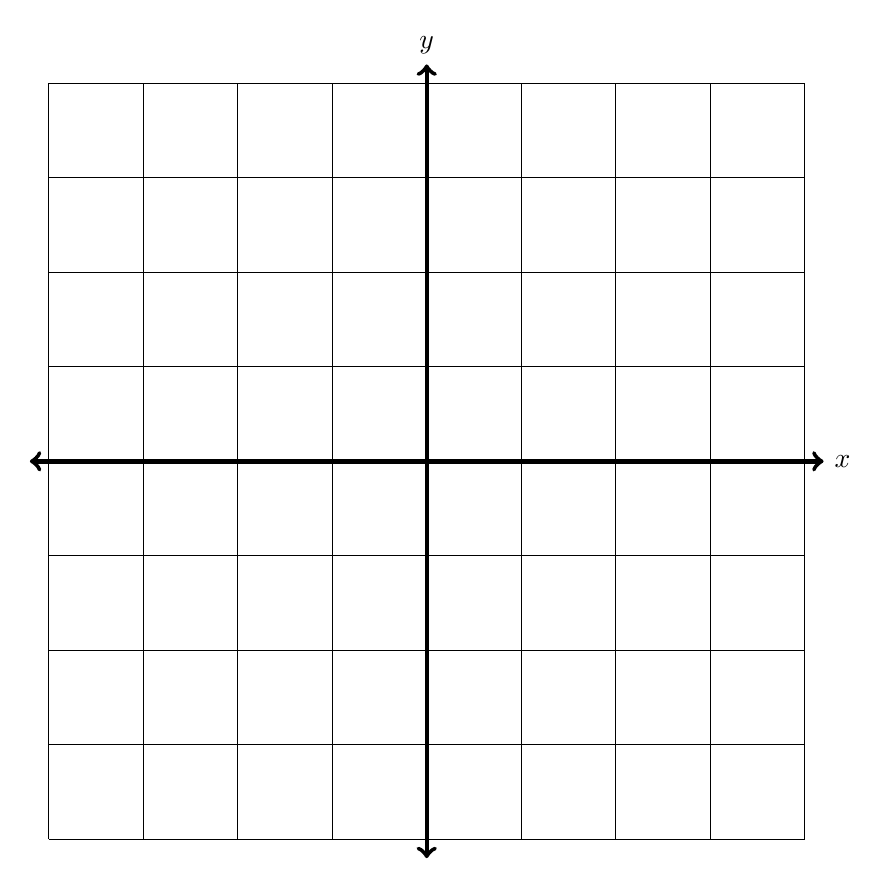
\begin{tikzpicture}[scale = 1.2]
      \draw (-4,-4) grid (4,4);
      \draw[ultra thick, <->] (-4.2,0)--(4.2,0);
      \draw[ultra thick, <->] (0,-4.2)--(0,4.2);
      \node at (4.4,0) {$x$};
      \node at (0,4.4) {$y$};
    \end{tikzpicture}

		\pagebreak
		\item (\textit{5 points})
    Consider the function $f(x)= 1 + \sqrt{x-2}$.
    Find the domain and range of this function.
    \\
    \textbf{(Hint: does it make sense to evaluate the function when $x=0$?
    Is it possible to get $0$ as an output?)}

    \vspace{3in}
    \item (\textit{1 point, extra credit})
    Water service costs a fixed amount each month, plus some price per unit of
    water used. Suppose that in January you use 100 units and get charged \$25,
    and in February you use 150 units and get charged \$35.
    Find an equation that describes the relationship between the amount of water
    used and the monthly bill.
  \end{enumerate}
\end{document}
